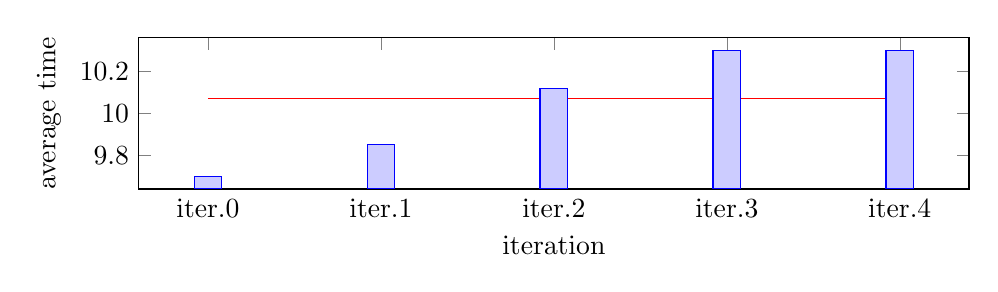
\begin{tikzpicture}
\begin{axis}[xlabel={iteration},
ylabel={average time},
symbolic x coords={iter.0,iter.1,iter.2,iter.3,iter.4},
width=\textwidth,
height=3.5cm,
xtick=data % important
]
%  \addplot+ [ybar,no markers,fill=blue!20,] coordinates { (naive,10.073)};
  \draw[red]
        (axis cs:iter.0,10.073)
        --  (axis cs:iter.4, 10.073)
    ;
 \addplot+ [ybar,no markers,fill=blue!20,] coordinates { (iter.0,9.701) (iter.1,9.854) (iter.2,10.118) (iter.3,10.301) (iter.4,10.301)};
\end{axis}
\end{tikzpicture}
